\setchapterpreamble[u]{\margintoc}
\chapter{A Brief Introduction}
\labch{intro}


\section{What We Talk About When We Talk About Urbit}
\labsec{urbittalk}

Urbit is a functional-as-in-language, network-first, compatibility-breaking
operation function (or hosted operating system).  But what does any of this mean?  As we explore Urbit software development throughout this book, keep in mind that every piece of Urbit aims to solve a ambitious battery of critical problems with the existing legacy World Wide Web.

\subsection{A Series of Unfortunate Events}

\paragraph{Centralization}.  For most contemporary corporations, whether enterprise-scale or startup, the driving factor for growth and revenue became the number of customers (users) they were able to attract to their platform or app.  Services like \texttt{del.icio.us} (founded 2003) and Flickr (founded 2004) betokened a wave of massive centralization, cemented by Facebook, Google, and Apple in the late aughts.  TODO XXX number of users on each in 2010

As users jostled onto burgeoning social media platforms, their patterns of behavior changed, and more and more social interactions of significance took place within "walled gardens," service platforms that interfaced only poorly with the exterior web.  Vendor lock-in and the nonportability of user data between platforms meant that consumer choice became a byword.  It became (and remains) difficult for any user to find out just what a corporation or even an app knows about them, particularly given the rise of surveilling cookies and data trackers.

The shift to mobile computing starting with the 2007 launch of Apple's iPhone drove a rise in cloud computing and cloud storage.  To many users, the data storage and access permissions on their data became largely illegible.  Sometimes this led to poor assumptions, such as that the custodial corporation would never allow a leak, or that the data would always be backed up safely.  As projects failed (like \texttt{del.icio.us}) or unilaterally changed policies (Tumblr), users permanently lost data.  Given the effort involved in curating tags, bookmarks, images, contacts, and research data, these outcomes frequently amounted in the loss of years of human effort.

\paragraph{Data leaks}.  During the 2000s and 2010s, data leaks became so common as to hardly merit notice.  As users flocked to corporate platforms for social media, publishing, photography, dating, and every other aspect of digital life, insufficient attention was given by corporations to both the practical security of user data and the potential fallout of leaks.  Data breaches grew in number ever year, and affected corporations of every size in every industry.

\begin{itemize}
  \item  2013:  Evernote, 50 million records
  \item  2014:  Ebay, 145 million records
  \item  2015:  Ashley Madison, 32 million records
  \item  2016:  Yahoo!, 1 billion records
  \item  2017:  Experian, 147 million records
  \item  2019:  Facebook, 850 million records
  \item  2019:  CapitalOne, 106 million records
\end{itemize}

("Records" does not equal "people" or even "accounts," of course, rendering these numbers mutually incommensurable.  Regardless, the scale staggers the mind.)  Sometimes these breaches were the result of clever social engineering; more frequently, someone forgot to properly salt password hashes or just stored or transmitted them in unencrypted plaintext.  Occasionally, the data were even just left available at a deprecated or forgotten API endpoint.  Identity security is challenging to get right, and those who had custody of user data were frequently subject to moral hazard.
%Data are from [Juliana de Groot, "The History of Data Breaches"](https://digitalguardian.com/blog/history-data-breaches) and [Wikipedia, "List of Data Breaches"](https://en.wikipedia.org/wiki/List_of_data_breaches).

\paragraph{The looming software stack}.  A combination of practical manufacturing limits ending Moore's law and a complexifying operating system and software stack led to a long-term stagnation in the perceived speed and fluidity of user experience with computers.  For the most part, even as multicore CPUs become more widespread, software bloat grows more acute with each new operating system version.  For many enterprise developers, there have been insufficient incentives to simplify software rather than to continue making it more complex.  Minimalist software by and large remained the demesne of hackers and code golf enthusiasts.

For instance,
TODO MS Word menu structure and file bloat
% https://winworldpc.com/product/microsoft-office/95

Even websites with visually minimalist aesthetics often presented
\citeauthor{Ceglowski2015}
a
- Optional Reading: \href{https://idlewords.com/talks/website_obesity.htm}{Maciej Cegłowski, "The Website Obesity Crisis"}

- Optional Reading: \href{https://idlewords.com/talks/build_a_better_monster.htm}{Maciej Cegłowski, "Build a Better Monster: Morality, Machine Learning, and Mass Surveillance"}

- Optional Reading: \href{http://marktarver.com/thecathedralandthebizarre.html}{Mark Tarver, "The Cathedral and the Bizarre"}


\paragraph{Security breaches}.  As the softwar stack grows, dependencies become opaque to downstream developers and users.  Upstream vulnerabilities have led to zero-day exploits and security breaches.  For instance, in 2014 the popular OpenSSL cryptography package had a bug of two years' standing revealed, Heartbleed.  This flaw in the Transport Layer Security (TLS) exposed memory buffers adjacent to

Instant-messaging protocols relying on the \texttt{libpurple} were impacted by an out-of-bounds write flaw in 2017, potentially permitting denial-of-service attacks or arbitrary code execution.

These two examples are not cherry-picked:  other examples abound.  The point stands that security breaches in the software stack render reliant software vulnerable in unpredictable ways.

\paragraph{Morbidity in open-source software projects}.  The rise of the free and open-source software (FOSS) movement has been enormously influential on software development and the end-user experience.  Spearheaded by Richard Stallman's GNU Project and Linus Torvalds' Linux operating system, FOSS rapidly overtook enterprise software offerings in terms of feature parity and upstream utilization.

Unfortunately, open-source software products are frequently broken in ways that are opaque to relatively nontechnical users:

\begin{enumerate}
	\item  FOSS can be construed as operating under a parasitic model.  Most real innovation happens outside of open-source projects, which are often clones of more successful proprietary software packages (LibreOffice/Microsoft Office, GIMP/Adobe Photoshop, Inkscape/Adobe Illustrator), and/or a clever way for a company to farm out development to free community labor (OpenOffice/Oracle, Ubuntu/Canonical, Darwin/Apple).  Thus even FOSS successes are often copies of proprietary antecedents.
  \item  FOSS suffers from [what one observer has dubbed](http://marktarver.com/thecathedralandthebizarre.html) "financial deficiency disease."  Even popular, well-used packages may have little oversight and funding for developers.  As alluded to above, OpenSSL was found in 2014 to have only one full-time developer despite being used by 66\% of Internet users.  Very few companies have succeeded in being FOSS-first (as opposed to FOSS-sometimes).
			%![](https://imgs.xkcd.com/comics/dependency.png)
  \item  FOSS has a hard time responding to customer demands.  The DIY ethos espoused by FOSS developers has often led to demurrage when features are requested.  This is the infamous response, "If you need it, why don't you build it yourself?"  Many users are unable to commit the time to implement the necessary features, and most FOSS projects do not have full-time developers and existing market dynamics sufficient to motivate rapid development.
\end{enumerate}

Even companies that loudly proclaimed support for "data liberation" used this FOSS openness like a lanternfish to later replace an open protocol (\eg~Google Talk) with a proprietary one (Google Hangouts).

Given the cascading stack of legacy software and strange interdependencies, actually getting the secure functionality a user wants often requires a proprietary platform anyway, undermining the aims of FOSS end-user applications and libraries.

\paragraph{Identity is cheap}.  Identity itself is cheap:  it costs botnets and spammers nothing to spin up new email addresses and new false identities.  Game-theoretically, spammers thrive in an environment where identity is close to free.

Identity is also dear:  losing a password in a breach can cause at best hours of resetting service logins and at worst the trauma and legal process of recovering from identity theft.

The foregoing summation may read as a bit emotional relative to what the reader is accustomed to reading in an academic textbook.  This is because the structure of our digital life matters as much as the content, and we have been ill-served to date by the incentives and powers that be.

Enter Urbit, stage right.

\subsection{Why Urbit}
\labsec{whyurbit}

\marginnote[2mm]{"Urbit is a clean slate reimagining of the operating system as an 'overlay OS', and a decentralized digital identity system including username, network address and crypto wallet."  (Tlon)}
The Urbit project intends to cut the Gordian knot of user autonomy and privacy.  To this end, the Urbit developers have articulated an approach prioritizing \emph{a legible future-proof program stack}, \emph{data security}, and \emph{cryptographic ownership}.  The ambitious scope of this project—and the evolution of the goals over the decade of the 2010s—has led many to have difficulty grasping what exactly Urbit is all about.  Urbit has been built to provide an Internet where communities can thrive without meddling or interference by third parties, and where what you build truly belongs to you.

\marginnote[2mm]{"[Urbit is] ultimately a hosted OS ([residing] on top of Linux) with an immutable file system with the additional purpose that you build applications distributed-first in a manner where clients store their own data."  ([`scarejunba`](https://news.ycombinator.com/item?id=21672481))}
Your Urbit is a personal server built as a functional-as-in-language operating system that runs as a virtual machine on top of whatever.  (Sometimes the developers refer to this arrangement as a "hosted OS," but they don't mean as in VMWare or VirtualBox or even containerization.)  The Urbit vision is the unification of services and data around a scarce futureproof identity on an innately secure platform.  Briefly put, Urbit requires you to have an \emph{Urbit OS} (which runs your code, stores your data, etc.) and an \emph{Urbit ID} (which secures your ownership of said code and data).

Urbit provides an excellent example of a visionary complex system which is radical (returning to the roots of computing) and forward-looking—and yet still small enough for us to grok all of the major moving parts in the system.  As a "hundred-year computer," Urbit represents how computing could work when computing power approaches negligible cost and bandwidth becomes effectively unlimited (or at least not limiting), instead focusing on the quality of user experience and user security.  We have found that Urbit is worthy of study in its own right as a compelling clean-state architecture embracing several innovative ideas at its base.

\paragraph{Legible future-proof program stack}.  The core of Urbit is an \emph{operating function}, or a functional-as-in-language operating system.  That is, there is a lifecycle function which receives a state and an event, processes the event, and yields a new state.

$$
L
(\sigma,\varepsilon)
\rightarrow
\sigma'
\textrm{.}
$$

This is called the Urbit OS to distinguish it from other aspects of the Urbit project when ambiguity is present.  The Urbit OS lifecycle function is written in a language called Nock and provides operational affordances through the Arvo operating core.  A schematic representation is frequently used:

![](repo:./img/00-urbit-all.png){: width=25%}

At its base, Arvo is an encrypted event log yielding a particular state.  The Nock virtual machine is like Urbit's version of assembler language, and it may in principle be implemented on top of any hardware.  Hoon is Urbit's equivalent of C, a higher-level language with useful macros and APIs for building out software.  Arvo runs atop these definitions.

The user can think of Urbit OS as a virtual machine which allows everything upstack to be agnostic to the hardware, and handles everything downstack.  Urbit has sometimes been described as an operating function, and this is what that means.  Everything is implemented as a stateful instance, called a "ship."

![](repo:./img/00-urbit-exploded.png){: width=50%}

\marginnote[2mm]{We will take a closer look at every part of this system in Chapter~\ref{kernel}.}
The vanes of Arvo provide services:  \ames~provides network interactivity, \clay~provides filesystem services and builds, \jael~provides cryptographic operations, and so forth.  On top of these are built the userspace apps.

![](repo:./img/00-arvo-exploded.png){: width=100%}

As a "hosted OS," Urbit doesn't seek to replace mainline operating systems.  Indeed, presumptively its Nock virtual machine could be run quite close to the bare metal, but Urbit itself would still require some provision of memory management, hardware drivers, and input/output services.  The overarching goal of the Urbit project is instead to replace the insecure messaging and service platforms and protocols used across the current web.

Urbit was designed on the principle that inheriting old platform code is a developer antipattern, given the complexities, vagaries, and vulnerabilities of legacy OSs.  In other words, things must break to be fixed.  Thus Urbit interfaces with other systems, but is a world unto itself internally.

\paragraph{Data security}.  TODO

\paragraph{Cryptographic ownership}.  We noted above that Urbit OS is an encrypted event log.  Urbit also acts as a universal \href{https://en.wikipedia.org/wiki/Single_sign-on}{single sign-on (SSO)} for the platform and for services instrumented to work with Urbit calls.  Since the Urbit address space is finite, each Urbit ID has inherent value within the system and should be a closely guarded secret.  An instantiation of your Urbit ID is frequently called a \emph{ship}, which lodges on your filesystem at a folder called a \emph{pier}.

\marginnote[2mm]{See Section~\ref{azimuth}~for more details.}
Following in the footsteps of other blockchain technologies, Urbit secures ownership of unique access points in the Urbit address space using Azimuth.  Currently Azimuth is deployed on top of the Ethereum blockchain.

Urbit IDs have mnemonic names attached to them, although fundamentally they are only a number in the address space.  For instance, one example address on Urbit is \texttt{~dopzod-binfyr}, the unique ID one user owns, corresponding to the 32-bit address \texttt{0xeb2a.5a32} in hexadecimal.

% Write like SeeTee shareholder letter but for Urbit, demolish all objections

On this network-oriented platform, users provide data to service endpoints, retaining their data rather than farming it out.  While no control can be exercised over data once sent out, a proposed reputation system can penalize bad actors in the system with reduced network access and other sanctions.

Let us posit a social operating system, or SOS;  a protocol for network-oriented platforms to utilize to ensure that user requirements are met securely.  If we enumerate user-oriented desiderata for a social operating system, surely the following must rank prominently:

TODO

\marginnote[2mm]{\citeauthor{Thompson1984}}
The system is designed to be transparent.  Something that runs on the Nock VM is of necessity open-source—no binary blobs!  (As with Ken Thompson's "Reflections on Trusting Trust", one can't necessarily trust what's below completely, but that's a problem with any system one did not build oneself from the bare metal up.)

\marginnote[2mm]{At this point, you may feel confused as to what exactly Urbit is.  That's understandable:  it's hard to explain a new system in full until it has started to manifest new and interesting features with broader repercussions.  For comparison, consider the following two interviews from much earlier in the history of the public Internet:

\begin{itemize}
	\item  \href{https://www.youtube.com/watch?v=gipL_CEw-fk}{Bill Gates on David Letterman, 1995} (an attempt to explain the Internet before almost anyone grokked it)
	\item  \href{https://www.youtube.com/watch?v=LaHcOs7mhfU}{David Bowie on the BBC, 1999} (a prophecy which grasps the essence without the technicality)
\end{itemize}

On this basis, it's safe to say that Gates got it, but Bowie ``got it.''  Their interlocutors did not.}
Identity on the current Web is frequently ephemeral and difficult to distinguish from spam.  Identity on Urbit is scarce and stable, much like moving into a house.  The SSO aspect of the system means that you have to remember and use many fewer passwords, and the cryptographic security layers means that as long as you treat your master key like your Bitcoin wallet you will have perpetual security.

The Urbit project does not completely solve all of these problems—for instance, pwned hardware—but it offers a reasonable set of solutions for many of the social and software issues raised by contemporary corporate practice on the World Wide Web.  Many think that it is better to attempt to fix the challenges of data control, privacy, and equity on the current web: \href{https://sovrin.org/}{Sovrin}, \href{https://webassembly.org/}{WebAssembly}, \href{https://ipfs.io/}{InterPlanetary File System}, \href{https://holochain.org/}{Holochain}, \href{https://blog.space.storage/posts/Introducing-Space}{Space}, and \href{https://scuttlebutt.nz/}{Scuttlebutt} each, in their own way, attack the same problems that Urbit seeks to solve, and each is worthy of the reader's further study.

All in all, Urbit like Bitcoin and (the best) blockchain applications seeks to securely deliver on the aims of the old Cypherpunk movement of the 1980s and 1990s:  digital security, digital autonomy.


\section{Azimuth, the Urbit Address Space}
\labsec{azimuth}



In \citeyear{Zooko2001}, digital cash pioneer Zooko Wilcox-O'Hearn postulated that a namespace cannot simultaneously possess three qualities:

\begin{enumerate}
	\item  distributedness ("in the sense that there is no central authority which can control the namespace, which is the same as saying that the namespace spans trust boundaries"),
	\item  security ("in the sense that name lookups cannot be forced to return incorrect values by an attacker, where the definition of "incorrect" is determined by some universal policy of name ownership"), and
	\item  human legibility (or interpretable by human users).
\end{enumerate}

This trilemma, dubbed Zooko's triangle, laid down a challenge to cryptographic researchers, who spent some effort to empirically refute the postulate.

In the case of Urbit,

% https://web.archive.org/web/20011020191610/http://zooko.com/distnames.html


\begin{marginfigure}[-5.5cm]
	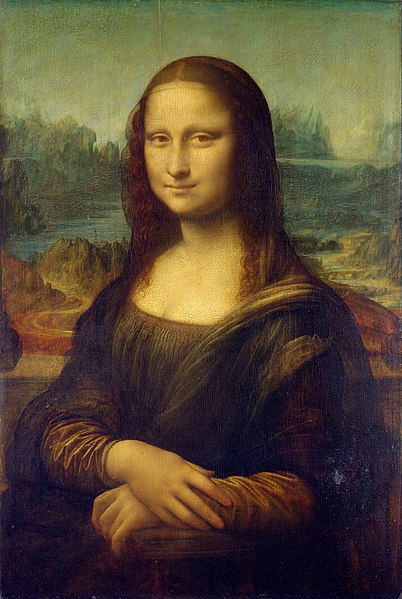
\includegraphics{monalisa}
	\caption[Sigils]{Some sigils\\
	\url{https://media.urbit.org/site/posts/essays/help-the-environment.jpg}}
	\labfig{marginsigils}
\end{marginfigure}

\section{A Frozen Operating System}
\labsec{frozen}

The philosophy underlying Urbit bears a strange resemblance to mathematics:  rather than running always as fast as one can to stay in the same place (a Red Queen's race), one should instead establish a firm foundation on which to erect all future enterprises.  In this view, the operating system should provide a permanently future-proof platform for launching your applications and storing your data—rather than a pastiche of hardware platforms and network specifications, all of that is hidden, "driver-like."  The OS should explicitly obscure all of that and no reaching beneath the OS should be allowed.

\marginnote[2mm]{Urbit frequently refers to its way of doing things as "Martian."}
From [the docs](https://web.archive.org/web/20140424223249/http://urbit.org/community/articles/martian-computing/):

\begin{quote}
Normally, when normal people release normal software, they count by fractions, and they count up. Thus, they can keep extending and revising their systems incrementally. This is generally considered a good thing. It generally is.

In some cases, however, specifications needs to be permanently frozen. This requirement is generally found in the context of standards. Some standards are extensible or versionable, but some are not. ASCII, for instance, is perma-frozen. So is IPv4 (its relationship to IPv6 is little more than nominal - if they were really the same protocol, they'd have the same ethertype). Moreover, many standards render themselves incompatible in practice through excessive enthusiasm for extensibility. They may not be perma-frozen, but they probably should be.

The true, Martian way to perma-freeze a system is what I call Kelvin versioning. In Kelvin versioning, releases count down by integer degrees Kelvin. At absolute zero, the system can no longer be changed. At 1K, one more modification is possible. And so on.
\end{quote}

\marginnote[2mm]{Urbit is not, of course, the only system to adopt an asymptotic approach to its final outcome.  \href{http://www.texfaq.org/FAQ-TeXfuture}{Donald Knuth, famous for many reasons but in this particular instance for the typesetting system \TeX, has specified that \TeX~versions incrementally approach $\pi$.}  \TeX~will reach $\pi$ definitively upon the date of Knuth's death, at which point all remaining bugs are instantly transformed into features and the version becomes $\pi$.  The current version of TeX is 3.14159265.}
In other words, Urbit is intended to cool towards absolute zero, at which point its specification is locked in forever and no further changes are countenanced.  This doesn't apply to everything in the system—"there simply isn't that much that needs to be versioned with a kelvin" (~nidsut-tomdun)—but it does apply to the most core components in the system.

\marginnote[2mm]{Think of the hypothetical structure of Jupiter:  clouds over a sea of metallic hydrogen over a diamond as big as Earth.
TODO image}
In this light, when we talk about Urbit we talk about three things:
\begin{enumerate}
	\item  Crystalline Urbit (the promised frozen core, 0K)
  \item  Fluid Urbit (the practice, mercurial and turbulent but starting to take shape)
  \item  Mechanical Urbit (the under-the-hood elements, still a chaos lurching into being, although much less primeval than before)
\end{enumerate}


\section{Developing for Urbit}
\labsec{developing}

The primary aim of this textbook is to expound Urbit in sufficient depth that you can approach it as an effective software developer.  We assume previous programming experience of one kind or another, not necessarily in a functional language.

Urbit development can be divided into three cases:

\begin{enumerate}
	\item  Kernel development
	\item  Userspace development, Urbit-side (\gall~and generators)
	\item  Userspace development, client-side (Urbit API)
\end{enumerate}

dojo ships fakezods

This guide focuses on getting the reader up to speed on the second development case early, then branches out into the two others.  With a solid foundation in \gall, the reader will be well-equipped to handle demands in either of the other domains.  We encourage the reader to approach each example and exercise in the following spirit:

\begin{enumerate}
  \item  Identify the input and outputs, preferably at the data type level and contents.
	\item  Reason analogically from other Hoon examples available in the text and elsewhere.
	\item  Create and complete an outline of the code content.
	\item  Devise and compose a suitable test suite.
\end{enumerate}


\section{Exercises}
\labsec{intro:exercises}

\begin{enumerate}
	\item  Obtain an Urbit ID and set up your Urbit OS.  Use the current installation procedure outlined at \href{https://urbit.org/}{\texttt{urbit.org}}.  You do not need to use a hosting service if you prefer to run Urbit on your own hardware, but maintaining your ship in an always-connected state will improve your experience.
	\item  Set up a fakezod for software development.
\end{enumerate}
